\hypertarget{_segmenter_8hpp}{
\section{Segmenter.hpp File Reference}
\label{_segmenter_8hpp}\index{Segmenter.hpp(153)@{Segmenter.hpp(153)}}
}


\subsection{Detailed Description}
Declaration of the class \hyperlink{class_segmenter}{Segmenter}. 



Definition in file \hyperlink{_segmenter_8hpp-source}{Segmenter.hpp}.

{\tt \#include $<$vector$>$}\par
{\tt \#include \char`\"{}Shape.hpp\char`\"{}}\par


Include dependency graph for Segmenter.hpp:\nopagebreak
\begin{figure}[H]
\begin{center}
\leavevmode
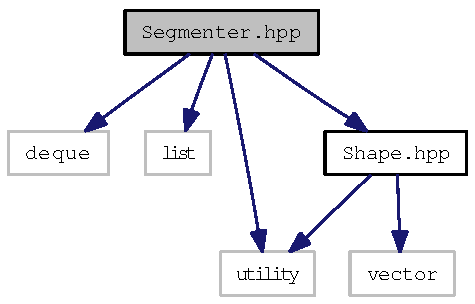
\includegraphics[width=86pt]{_segmenter_8hpp__incl}
\end{center}
\end{figure}


This graph shows which files directly or indirectly include this file:\nopagebreak
\begin{figure}[H]
\begin{center}
\leavevmode
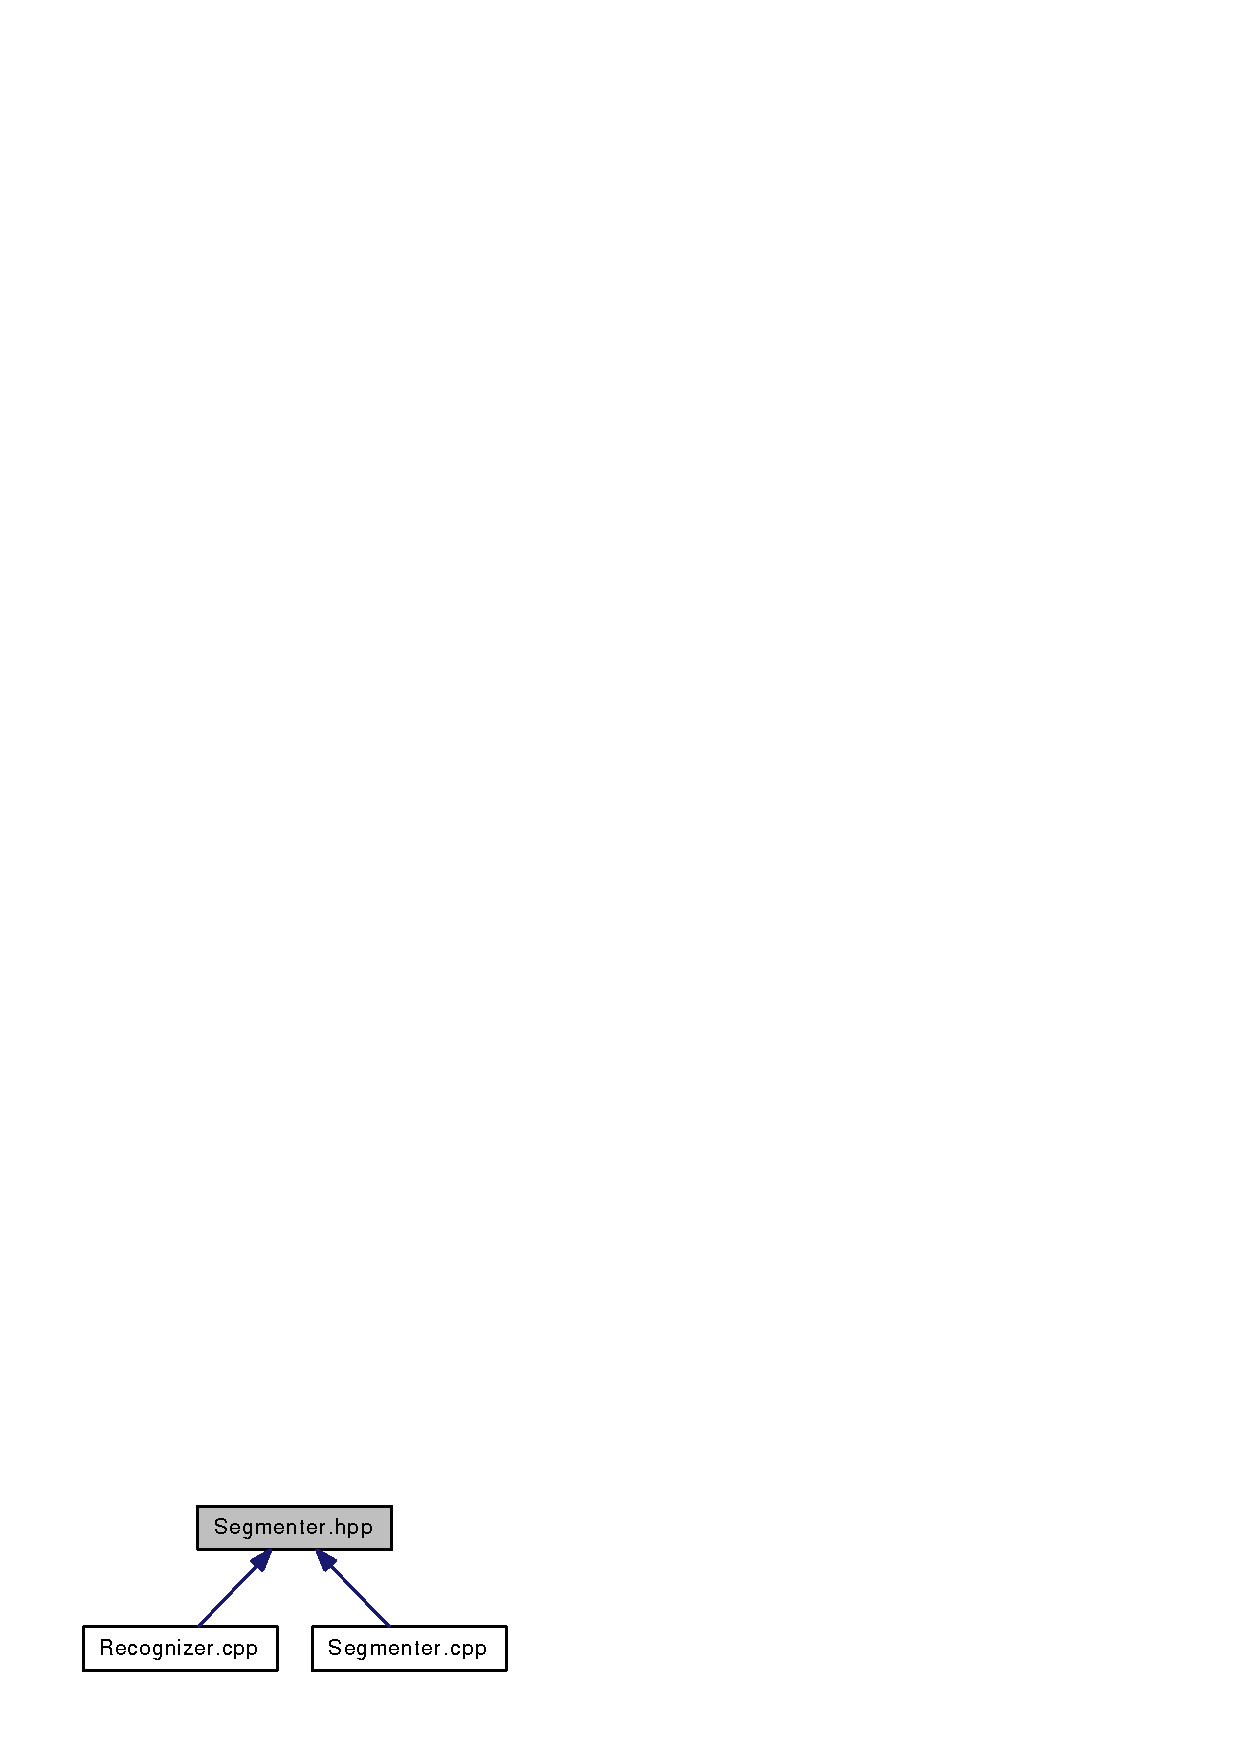
\includegraphics[width=123pt]{_segmenter_8hpp__dep__incl}
\end{center}
\end{figure}
\subsection*{Data Structures}
\begin{CompactItemize}
\item 
class \hyperlink{class_segmenter}{Segmenter}
\begin{CompactList}\small\item\em \hyperlink{class_segmenter}{Segmenter} of the OCR process. \item\end{CompactList}\end{CompactItemize}
